% Options for packages loaded elsewhere
\PassOptionsToPackage{unicode}{hyperref}
\PassOptionsToPackage{hyphens}{url}
%
\documentclass[report,gutter=10mm,fore-edge=10mm,uplatex,dvipdfmx]{jlreq}

\usepackage{lmodern}
\usepackage{amssymb,amsmath}
\usepackage{ifxetex,ifluatex}
\usepackage{actuarialsymbol}
\usepackage[]{natbib}
\RequirePackage{plautopatch}

% maru suji ① etc.
\usepackage{tikz}
\newcommand{\cir}[1]{\tikz[baseline]{%
\node[anchor=base, draw, circle, inner sep=0, minimum width=1.2em]{#1};}}

\usepackage{comment}

\begin{comment}

\ifnum0\ifxetex1\fi\ifluatex1\fi=0 % if pdftex
  \usepackage[T1]{fontenc}
  \usepackage[utf8]{inputenc}
  \usepackage{textcomp} % provide euro and other symbols
\else % if luatex or xetex
  \usepackage{unicode-math}
  \defaultfontfeatures{Scale=MatchLowercase}
  \defaultfontfeatures[\rmfamily]{Ligatures=TeX,Scale=1}
\fi
% Use upquote if available, for straight quotes in verbatim environments
\IfFileExists{upquote.sty}{\usepackage{upquote}}{}
\IfFileExists{microtype.sty}{% use microtype if available
  \usepackage[]{microtype}
  \UseMicrotypeSet[protrusion]{basicmath} % disable protrusion for tt fonts
}{}
\makeatletter
\@ifundefined{KOMAClassName}{% if non-KOMA class
  \IfFileExists{parskip.sty}{%
    \usepackage{parskip}
  }{% else
    \setlength{\parindent}{0pt}
    \setlength{\parskip}{6pt plus 2pt minus 1pt}}
}{% if KOMA class
  \KOMAoptions{parskip=half}}
\makeatother
\usepackage{xcolor}
\IfFileExists{xurl.sty}{\usepackage{xurl}}{} % add URL line breaks if available
\IfFileExists{bookmark.sty}{\usepackage{bookmark}}{\usepackage{hyperref}}
\hypersetup{
  hidelinks,
  pdfcreator={LaTeX via pandoc}}
\urlstyle{same} % disable monospaced font for URLs
\usepackage{longtable,booktabs}
% Correct order of tables after \paragraph or \subparagraph
\usepackage{etoolbox}
\makeatletter
\patchcmd\longtable{\par}{\if@noskipsec\mbox{}\fi\par}{}{}
\makeatother
% Allow footnotes in longtable head/foot
\IfFileExists{footnotehyper.sty}{\usepackage{footnotehyper}}{\usepackage{footnote}}

\end{comment}
%\makesavenoteenv{longtable}
\setlength{\emergencystretch}{3em} % prevent overfull lines
\providecommand{\tightlist}{%
  \setlength{\itemsep}{0pt}\setlength{\parskip}{0pt}}
\setcounter{secnumdepth}{-\maxdimen} % remove section numbering

\author{kazuyoshi}
\date{}

\newcommand{\problem}[1]{\subsubsection{#1}\setcounter{equation}{0}}
%\newcommand{\answer}[1]{\subsubsection{#1}}
\newcommand{\answer}[1]{\subsubsection{解答}}

%Pdf%\newcommand{\wakumaru}[1]{\framebox[3zw]{#1}}
\newcommand{\wakumaru}[1]{#1}






\begin{document}

\chapter{保険1第1章 営業保険料}

\section{1.2 営業保険料決定の際に考慮すべき点}

\subsection{営業保険料決定の際に考慮すべき事項4つ}

\problem{ H27 問3 (1) 1,2; H19 問3 (1)1; H17 問3 (2)1}

\begin{enumerate}
    \tightlist
\item  十分性
  \begin{itemize}
    \tightlist
  \item
    最も重要。
  \item
    会社の最終的な支払い能力を決定する。
  \item
    契約者からの直接の収入
  \item
    十分な検証が必要
  \end{itemize}
\item
  公平性

  \begin{itemize}
    \tightlist
  \item
    契約者のために考慮すべき点
  \item
    理論的に完璧な公平性を実現する必要はなく、
  \item
    実務の簡素化を念頭におきつつ、
  \item
    保険料における公平性の問題を考えるべき

    \begin{itemize}
    \tightlist
    \item
      個人保険の保険料は、保険種類・年齢・性別によって異なるのが一般的

      \begin{itemize}
      \tightlist
      \item
        団体保険や各種特約も同様であるべきか、
      \item
        年齢は歳別か群団料率か、といった点もある
      \end{itemize}
    \end{itemize}
  \end{itemize}
\item
  収益性

  \begin{itemize}
  \tightlist
  \item
    有配当の相互会社であれば、十分性が満たされていれば、収益性はさほど重要ではないという考えもある
  \item
    無配当の株式会社であれば、収益性の検証の重要性はより高まる
  \end{itemize}
\item
  標準責任準備金制度との関係

  \begin{itemize}
  \tightlist
  \item
    営業保険料の計算基礎率は各社の判断により決定すべき
  \item
    十分性を慎重に検証した上で、より低廉な営業保険料を設定することも可能

    \begin{itemize}
    \tightlist
    \item
      責任準備金の積立水準は収益の認識時期に影響するのみ

      \begin{itemize}
      \tightlist
      \item
        十分性の指標として保険期間満了時までの収益の単純合計を見るとすれば、
      \end{itemize}
    \item
      保険期間途中では積立負担が大きくなる

      \begin{itemize}
      \tightlist
      \item
        予定利率が標準利率より高い場合、特に一時払契約においては、契約初期にかなり大きな積立負担が発生
      \item
        積立負担を当該保険群団で賄えない場合は、

        \begin{itemize}
        \tightlist
        \item
          他の保険群団の剰余
        \item
          会社勘定(内部留保)で立て替えることになる。
        \end{itemize}
      \item
        標準責任準備金の積立は一種の初期投資、内部留保の水準から容認できる範囲で行うという考え
      \item
        結果として保険料の不足を引き起こす恐れもある
      \end{itemize}
    \item
      十分性が保たれているかどうかの判断には困難がつきまとうため、慎重に検討する必要がある
    \end{itemize}
  \end{itemize}
\end{enumerate}

\problem{2020  生保1問題 2(1)①②}
① 営業保険料を決定する際に考慮すべき点のうち、標準責任準備金制度との関係について簡潔に説明しなさい。(6点)

② 営業保険料の引下げに関して、次の(ア)、(イ)の各問に答えなさい。なお、解答にあたって、付加保険料体系は、予定新契約費が保険金比例と保険料比例、予定維持費が保険金比例、予定集金費が保険料比例とする。

(ア)付加保険料を引き下げた場合、平準払の終身保険において引下げ前には生じていなかった
契約初期の標準責任準備金の大きな積増負担が発生することがある。考えられる要因を簡
潔に説明しなさい。(2点)

(イ)予定利率を引き上げた場合、平準払の定期保険において営業保険料が引き下がらず、引上
げになることがある。考えられる要因を簡潔に説明しなさい。(2点)

\answer{解答}

①
\begin{itemize}
 \item  標準責任準備金の評価基礎率(以下、
 「標準基礎率」)は、平成 8 年大蔵省告示第 48 号にて水準等が
 定められているが、営業保険料の計算基礎率(以下、
 「保険料基礎率」)は各社の判断で決定すべき
 ものであり、必ずしも標準基礎率にあわせる必要はなく、十分性を検証したうえで、より低廉な営
 業保険料を各社設定すればよい。
 \item  保険料基礎率と標準基礎率に差があり、保険料基礎率より標準基礎率で計算した責任準備金の水準
 の方が大きい場合、保険期間満了時までの収益の単純合計には影響しないものの、保険期間の途中
 で積立負担が生じる。
 \item  一時払においては予定利率が標準利率より高い場合、契約初期にかなり大きな積立負担が発生する
 可能性がある。
 \item  平準払(の貯蓄性商品)においては、標準基礎率による純保険料が、保険料計算基礎率による営業
 保険料を上回っている場合、この積立負担が大きくなる可能性がある。
 \item  この積立負担は当該保険群団でセルフサポートすることが望ましいが、積立負担を保険群団で賄え
 ない場合、他の保険群団の剰余または内部留保で立て替えることになる。その水準にもよるが恒常
 的に立替えが必要な状態は好ましくない。
 \item  標準責任準備金の積立は、将来の収益を得るために会社が内部留保の水準から容認できる範囲の初
 期投資を行うという考え方もあるが、この場合、結果として保険料の不足を引き起こすおそれもあ
 ることから、保険料の十分性が保たれているかどうかについて、慎重に検討する必要がある。
 \item  過去、標準利率引き下げのタイミングで予定利率の改定が行われることが多かったことを踏まえる
 と、標準基礎率は保険料基礎率に相応に影響を与えるものと考えられる。
\end{itemize}

②(ア)

営業保険料が標準基礎率に基づく平準純保険料より小さい場合、これを標準責任準備金の計算にお
ける「将来の保険料」として用いなければならなく、契約初期の平準払いであっても標準責任準備金
が0付近にならないため。

(イ)

若齢・払込期間が短期の場合に、予定利率の上昇によって純保険料が小さくなる一方で、年金現価
が小さくなるために営業保険料に含まれる平準化された保険金比例の予定新契約費が大きくなる影
響の方が大きく、営業保険料全体が増加している。
※②はあくまで解答例であり、この他にも正しい記述に対して適宜加点した。

\problem{H27 生保1問題 3(1)①②}
平準払の貯蓄性商品の予定利率設定について、次の1.,2.の各問に答えなさい。

\begin{enumerate}
 \item  営業保険料決定の際に考慮すべき事項である「十分性」「公平性」「収益性」について、それぞれ簡潔に説明しなさい。 (4 点)
 \item 「営業保険料の計算基礎率」と「標準責任準備金の評価基礎率」の関係について簡潔に説明しなさい。 (6 点)
\end{enumerate}

\answer{解答}
\begin{enumerate}
 \item 営業保険料決定の際に考慮すべき事項である「十分性」「公平性」「収益性」
\begin{itemize}
 \item [十分性]十分性は保険金等の支払能力を営業保険料収入で十分に賄うことができるか、つまりはセルフサポートできているかということである。予定利率の場合は、想定される運用利回りに対して十分なマージンを確保しているかが重要である。
 \item [公平性]公平性は契約者のために考慮すべき点であるが、一方で実務の簡素化も念頭に考える必要がある。具体的には保険技術的公平性を充足しているか、つまり同料率の保険群団は、同程度のリスクであるかや、社会的に受け入れられるか(社会的公平性)という視点で見ることになる。ただし、完璧な公平性の実現は困難であるため、一定程度、簡素化が求められる。
 \item [収益性]収益性は、要は設定した営業保険料により会社にどの程度の収益性をもたらすかという視点である。収益性を確認する際には、予定利率を十分なマージンをもって設定した場合、販売量が犠牲になるなど、価格と販売量のトレードオフに留意する必要がある。また、収益性の捉え方は会社形態・配当方式により若干意味合いが異なるという点もある。例えば有配当の相互会社であれば十分性を満たした料率を設定し、収益を配当で還元するという前提のもとに、あまり収益性を重要視しないことも考えられよう。しかし、近年は相互会社も EV を開示するなど、会社形態による差異は少なくなっているとも考えられる。
\end{itemize}
 \item 「営業保険料の計算基礎率」と「標準責任準備金の評価基礎率」の関係
\begin{itemize}
 \item 営業保険料の計算基礎率(以下、「保険料基礎率」)は各社の判断で決定すべきものであり、必ずしも標準責任準備金の評価基礎率(以下、「標準基礎率」)にあわせる必要はない。
 \item 一方で、標準基礎率は大蔵省告示第 48 号に基づき定められるものである。
 \item 保険料基礎率による予定利率が標準利率を上回っている場合、保険期間満了時までの収益の単純合計には影響しないものの、契約初期に積立負担が生じる。
 \item 特に平準払の貯蓄性商品においては、標準基礎率による純保険料が、保険料計算基礎率による営業保険料を上回っている場合、この積立負担が大きくなる可能性がある。
 \item この積立負担は当該商品区分でセルフサポートすることが望ましい。
 \item 積立負担を保険群団で賄えない場合、他の保険群団の剰余または内部留保で立て替えることになる。
 \item 過去においては、標準利率引き下げのタイミングで予定利率の改定が行われることが多かったことを踏まえると、標準基礎率は、保険料基礎率に相応に影響を与えるものと考えられる。
\end{itemize}
\end{enumerate}

\problem{H19 問3 (1)①}

営業保険料決定の際に考慮すべき点のうち、「十分性」ならびに「標準責任準備金制度との関係」について簡潔に説明せよ。

\answer{解答}

\begin{itemize}
\tightlist
\item
  十分性

  \begin{itemize}
  \tightlist
  \item
    最も重要な点

    \begin{itemize}
    \tightlist
    \item
      会社の最終的な支払能力が決定される
    \item
      契約者からの直接の収入
    \end{itemize}
  \item
    十分な検証が必要

    \begin{itemize}
    \tightlist
    \item
      保険期間が長期にわたること
    \item
      利源分析等を参考に各基礎率の十分性についても検証し、
    
      \item
      その他の営業保険料決定の際に考慮すべき点とのバランスにも留意する必要がある。
    \end{itemize}
  \end{itemize}
\item
  標準責任準備金制度との関係

  \begin{itemize}
  \tightlist
  \item
    営業保険料の計算基礎率は、各社が各社の判断により決定すべきものであり、

  \item
      必ずしも標準責任準備金の評価基礎率(以下標準基礎率)にあわせる必要はない。

      \begin{itemize}
      \tightlist
      \item
        十分性を慎重に検証
      \item
        低廉な営業保険料を設定

        \begin{itemize}
        \tightlist
        \item
          保険期間の途中では積立負担が発生する。

          \item
            営業保険料およびその内訳である純保険料と対応しない
          \item
            その保険群団でまかなえない場合は、立て替えることになる。

                \item
              他の保険群団の剰余
            \item
              会社勘定(内部留保)
              \item
            恒常的に立替えが必要な状態は好ましくないと言える。
          \item
            内部留保の水準から容認できる範囲の初期投資
          \item
            結果として保険料の不足を引き起こす恐れ
          
        \end{itemize}
      \end{itemize}
    \item
      アクチェアリーとしで慎重に検討する必要がある。
    
  \end{itemize}
\end{itemize}

\section{1.3 営業保険料決定の諸要素}
\subsection{死亡率}

\problem{2022 生保1問題 1(6)(ア)}
次の図は厚生労働省が公表する「平成 30 年 我が国の人口動態」より「主な死因別にみた死
亡率の年次推移」である。グラフが示す死因について、次の①~③の空欄に当てはまる最も適
切なものをそれぞれ次の選択肢の中から1つ選び、記号で答えなさい。なお、①~③を含む全
ての空欄には選択肢のいずれかが当てはまる。(3点)

       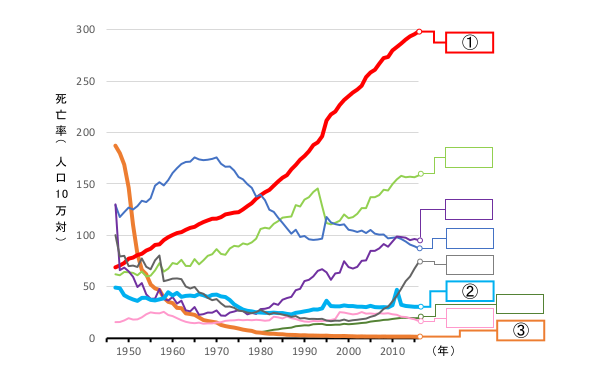
\includegraphics[scale=1]{images/Prob2022-1-1-6-a.png}


※上記の死亡率は年齢調整前死亡率である。年齢調整とは、年次推移において人口の年齢構成
の差異を取り除くために、ある(一時点の)基準人口を用いて計算することを指す。

【選択肢】
(A)不慮の事故 (B)老衰 (C)自殺
(D)がん (E)脳卒中 (F)結核
(G)肺炎 (H)心臓病 (I)腎不全

\answer{解答}
① D 
第1位は、がん
② A 
2011年東日本大震災影響で不慮の事故
③ F
1950年第1位で現在はほぼ0.結核。

\problem{2021 生保1問題 2(1)}

第三分野標準生命表2018の作成過程を簡潔に説明しなさい。
なお、第三分野標準生命表2007の作成過程からの主な変更点とその変更理由にも触れること。
\answer{解答}

まず、第三分野標準生命表2018(以下、
「生命表2018」)の基礎データとして第 21 回生
命表を用いる。

第三分野標準生命表2007(以下、「生命表2007」)作成時は、第三分野は特約形式で死亡
保障性商品に付加される割合が高かったことから、基礎データに生保標準生命表2007(死亡保
険用)とあわせて死亡保険の経験死亡率(業界データ)を用いたが、生命表2018では契約形態
の変化(主契約・単品化)の実態や死亡保険との診査手法の相違、同じ生存リスクに対応する年金
開始後用との整合性等を踏まえて変更している。このため、生命表2007で行っていた若齢部分
の補整や基礎データの截断を生命表2018では行っていない(基礎データで既に行われている)
。

次に、この基礎データに対し、基礎データの年度以降の死亡率の改善状況や米国における標準生
命表の作成方法等を踏まえて、標準生命表の適用年までの死亡率改善を反映することを生命表20
18で導入している。具体的には国民死亡率の実績が判明している 2010 年から 2015 年の簡易生命
表を踏まえて、2015 年までの年平均改善率を男性 2.5\%女性 2.0\%と推計し5年分を、国民死亡率の実
績が判明していない 2015 年から標準生命表が適用される 2018 年までは国立社会保障・人口問題研
究所の将来推計人口の結果を踏まえて、年平均改善率を男女ともに 1.0\%と推計し3年分を、それぞ
れ反映して補整前死亡率としている。

最後に、補整前死亡率に対し、単年度のブレへの対応、母数の差による違いの吸収、基礎データ
を国民表とすることへの対応、将来の死亡率変動への対応などの観点から数学的危険論に基づいて
補整を行う。具体的には標本数が十分に大きければ標本死亡率は正規分布に従うとして補整前死亡
率から2σを減じた(ただし補整前死亡率の 70%を下限とし、さらに生命表2018では特に高齢
部分の「将来の死亡率変動への対応」を図る観点から上限 85%も追加した。)
。なお、この補整で用
いる標本の大きさは生命表2018では直近実績の各社の契約件数も踏まえて男女各々100 万件(生
命表2007では 400 万件)としている。

また、生命表2007作成時に行った死亡率曲線の平滑化(グレビルの多項式による補整)や高
齢の補外(ゴムパーツメーカムの法則)は、生命表2018の基礎データ自体に既に行われている
ため行っていない。なお、生命表2007は死亡率に高度障害を含むのに対し、生命表2018は
含まないことも異なる点である。

\problem{H11 問1(改)}

次の①~⑤を適当な語句で埋めよ。
生保標準生命表\sout{1996}2018(死亡保険用)の作成概要は以下のとおりである。 

\begin{center}
 基礎データの収集→①の決定→②-1→ ②-2→ ②-3(この中に1,2,3次)→ 標準生命表
\end{center}

①の決定においては、標準生命表に求められる、死亡率の安定性・安全性の確保および経験死亡率の③の実態を勘案し、④および⑤を決定した。

\answer{解答}
①粗死亡率 ②-1 若年齢の補整  ②-2 死亡率改善の反映 ②-3 補整 ③選択効果④,⑤観察年度、截断年数

\problem{H16 生保1問題 1(3)1(改)}

生保標準生命表 \sout{1996}2018(死亡保険用)に関する次の①②について答えよ。

\begin{itemize}
\tightlist
 \item [①]  ア)からウ)について正しいものには○、誤りのあるものには×を解答欄に付けよ。
\begin{itemize}
\tightlist
 \item [ ア)]生保標準生命表 \sout{1996} 2018 は、標準責任準備金の計算に使用される予定死亡率であり、生命保険協会が作成した。
 \item [ イ)]粗死亡率の基礎データは、厚生労働省から提供を受けた簡易生命表である。
 \item [ ウ)]観察年度は選択効果を排除するため、\sout{1989~91} 2008,2009,2011 年度とした。
\end{itemize}
 \item [②] 下に示した(a)から(d)のグラフのうち(エ)(オ)に当てはまる記号を解答欄に記せ。
 0 歳から 50 歳の死亡率をグラフ表示したとき、男子の死亡率の特徴を最もよくとらえているグラ
 フは (エ) である、また女子の死亡率の特徴を最もよくとらえているグラフは (オ) である.

       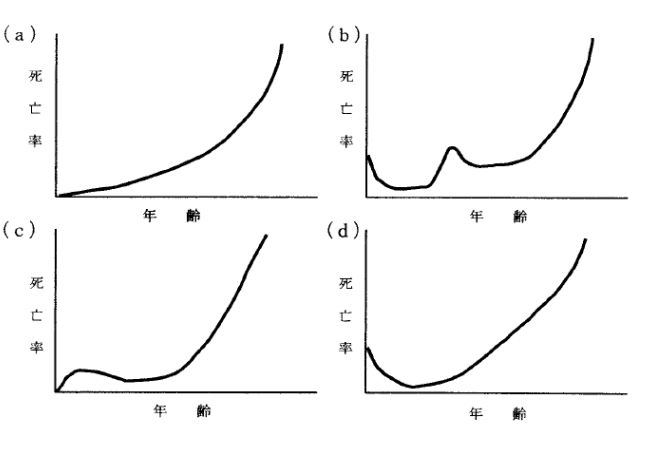
\includegraphics[scale=0.25]{images/probH161-1-3.png}

\end{itemize}


\answer{解答}

\begin{itemize}
\tightlist
 \item [①]
\begin{itemize}
\tightlist
 \item [ア)] × 生命保険協会→公益社団法人 日本アクチュアリー会
 \item [イ)]×厚生労働省から提供を受けた簡易生命表→生命保険協会にてまとめた生命保険会社の実績
 \item [ウ)]×選択効果を排除するためのものは、截断年数。
\end{itemize}
 \item [②]
\begin{itemize}
\tightlist
 \item 男子b:誕生直後が高く、20歳くらいで跳ね上がる(自動車事故?)
 \item  女子d:誕生直後が高い
\end{itemize}
\end{itemize}


\problem{H13 問1 (9)1(改)}

生保標準生命表\sout{1996} 2018 (死亡保険用)では、截断年数については以下のとおり設定した。なぜこのような截断年数を設けたのか、「截断年数」自体の説明も含め簡潔に説明せよ。

\begin{tabular}[t]{|c|c|c|}
\hline
 & 男子 &女子 \\
\hline
 1年截断& 1--19歳&1--4歳 \\
 2年截断& 20--24歳&5--24歳 \\
 3年截断& 25--29歳&25--29歳 \\
 4年截断& 30--34歳&30--34歳 \\
 5年截断& 35--39歳 & -- \\
 6年截断&  -- & 35--39歳 \\
 7年截断& 40--44歳   & 40--44歳 \\
 8年截断& 45--49歳   & 45--49歳 \\
 9年截断& --歳   & --歳 \\
 10年截断& 50歳--  & 50歳-- \\
\hline
\end{tabular}
( 0歳は初年度)

\answer{解答}
経験表作成の際、選択効果を排除し死亡率の安全性を確保するため、契約当初数年のデータを除外して作成するが、その除外期間を裁断年数という。

年齢群団間で選択効果に差が認められる点を考慮し、年齢別に1年裁断から10年裁断とし、男女間でも選択効果に差異が認められたことから、同じ裁断年数でも男女間で適用年齢に差異を設けた。
ただし、裁断年数を長くずれは安全な死亡率が作成できるわけではなく、裁断年数を長くした場合その部分のサンプルが少なくなることからかえって死亡率データとしての信頼性が減少する。
截断の上限年数は、前回作成時は5年としていたが、近年の実績では経過10年までは選択効果が認めらえることを踏まえ10年とした。

\problem{H29 問1 (4)}

生保標準生命表 2007(年金開始後用)は、第 19 回生命表(2000年)を基礎表とした上で、主に次のような処理を行って死亡率の安定性・安全性を加味している。
\begin{itemize}
\tightlist
\item
  将来の死亡率改善
\item
  ①の除去
\item
  将来死亡率の推定

今後も、上記「将来の死亡率改善」で求めた改善率で毎年死亡率が改善していくとして、将来の死亡率を推定する。推定する「将来」としては、原則として 1960 年生まれの人が各年齢に達する年とし、第 19 回生命表の死亡率に、2000 年からその「将来」までの年数だけの死亡率の改善を加えたものを、「将来の死亡率」とする。


ただし、最低でも②年分の死亡率の改善を見込むこととする。
\item
     生存リスク方向への補整
\end{itemize}
「単年度のブレへの対応」、「改善率の見込み差異の吸収」、「母数(会社規模)の差による違いの吸
収」、「③の違いの吸収」、「元データを国民表とすることへの対応」という観点から、死亡率の安
全性を目的として、改善率反映後の死亡率に④\%が乗じられている。

なお、生保標準生命表 2007(年金開始後用)における男性 60 歳の死亡率は⑤である。


〔⑤の選択肢〕
(A) 0.00006 (B) 0.00064
(C) 0.00642
(D) 0.06472
===

\answer{解答}

① コーホート効果 ② 20 ③ 代表生年 ④ 85 ⑤ C およその水準 0.64\%

\problem{H17 問1(3)(改)}

生保標準生命表\sout{1996} 2007(年金開始後用)死亡率の作成方法について、次の①~④の空欄を適当な数値または数式で埋めよ。

生保標準生命表 2007 (年金開始後用)死亡率は、第 15回生命表(1980年)と第 19 回生命表(2000年)とから将来の死亡率の改善を見込んで作成されたものである。
\begin{enumerate}
 \item 人口動態統計より性別・5歳群団別・死因別に年平均改善率を算出
\begin{itemize}
 \item 死因を8通りとした
 \item ICD(国際疾病分類)変更等の影響を除外するため、以下のとおり算出
\begin{itemize}
 \item [$R_1$]:1995年→2000年の5年間の年平均改善率(幾何平均)
 \item [$R_2$]:1980年→1993年の13年間の年平均改善率(幾何平均)
 \item [$R$]:求める年平均改善率
\end{itemize}

$R_1,R_2$の計算は(m>nとして)、
n年度生命表(死因・性・年齢別、以下同様)の x 歳の死亡率を\(q_x^{(n)}\)、
m年度生命表のそれを\(q_x^{(m)}\)とし改善率を求めると、1年あたりの改善率\(r_x\)= ① となる。

更に以下の算式で Rを求める。
$$
(1-R_1)^5\times(1-R_2)^{13} = (1-R)^{18}
$$

\end{itemize}

今後もこの改善率で毎年死亡率が改善していくとして将来の死亡率を推定する。推定する「将来」としては、原則として1960年生まれの人が各年齢に達する年とし、第 19 回生命表の死亡率に、2000年からその「将来」までの年数だけ改善を加えたものを「将来の死亡率」とする。(ただし、最低20 年分 の改善を見込む)

 \item 1で求めた年平均改善率を用いて、5歳群団の中央年齢の将来死亡率を死因別に予測
\begin{itemize}
 \item 代表生年として1960年
 \item 改善率がマイナスとなっている死因は改善率を0とした
\end{itemize}
 \item 2で求めた死因別死亡率の合計値と2000年の死亡率から死因合計の年平均改善率を算出
 \item 3で求めた中央年齢の年平均改善率を、年齢間で直線補間することにより各年齢の年平均改善率を算出
\end{enumerate}

各年齢における死亡率の改善を見込む年数は下表のとおりとなる。

\begin{tabular}[]{|c|c|c|}
\hline
年齢 & 推定する「将来」 & 死亡率の改善を見込む年数\\
60 歳 & 2020 年 & 20 年\\
70 歳 & ②年 & ③年\\
\hline
\end{tabular}

60 歳の死亡率の推定値は、\(q_x^{(19)}\)、\(r_{60}\)
を使用し④と計算される。
このようにして求めた将来の死亡率について、死亡率を滑らかにするための補整と高年齢での補外を行ったものを年金開始後死亡率としている。

===
\answer{解答}

① \(1-\{q^{(m)}/q^{(n)}\}^{1/(m-n)}\);
q比率を(1980-1955=)25年幾何平均。改善率とするため1から減算

② 2030;
基準年2000に、30年足す 

③ 30

④ \(q^{(19)}_{60}\cdot(1-r_{60})^{20}\);
改善率を1から減算したものを20乗

\problem{H12 問1(9)(改)}

生保標準生命表 \sout{1996} 2007 の年金開始後用死亡率の作成過程を簡潔に説明せよ。

===

\answer{解答}

\begin{enumerate}
\tightlist
\item
  基となる死亡率として、第19回生命表(2000年)の死亡率を用いる。
\item
  第19回生命表(2000)を第15回生命表(1980)と比較し、男女別・5歳群団別・死因別の死亡率改善状況を用いて、死亡率が1年当たりどれだけの割合で減少しているか(改善率)を求める。
\item
  今後も2.で求めた改善率で毎午死亡率が改善していくとして、5歳群団の中央年齢の将来死亡率を死因別に予測する。(推定する「将来」としては、原則として1960年生まれの人が各年齢に達する年とする。ただし、60歳以下の年齢については、推定する「将来」を2020年とする。)
\item
     3.で求めた死因別死亡率の合計値と2000年の死亡率(死因合計)から死因合計の年平均改善率を算出
 \item 
       4. で求めた中央年齢の年平均改善率を、年齢間で直線補間することにより各年齢の年平均改善率を算出。\\
       男子の45歳から52歳については、コーホート効果を除去するために、44歳と53歳の年平均改善率を直線補間
\end{enumerate}


\problem{2019 問1 (1)}

第三分野標準生命表 2018
の作成過程について、次の①~⑤に適切な語句を記入しなさい。

\begin{itemize}
\tightlist
\item
  基礎データの決定\\
  第三分野保険の契約形態の変化(主契約・単品化)、死亡保険との診査手法の相違、同じ生存リスクに対応する年金開始後用との整合性等を踏まえ、基礎データとして①の死亡率を用いることとした。なお、第三分野標準生命表2018
  は②を含まない死亡率であるが、第三分野標準生命表2007は②を含む死亡率である。
\item
  死亡率改善の反映\\
  死亡率の改善状況等を踏まえ、基礎データに標準生命表の適用年までの死亡率改善を反映したものを補整前死亡率とした。具体的な改善率は、国民死亡率の実績が判明している
  2015 年までは、男性が年 2.5\%、女性が年 2.0%であり、2015
  年から標準生命表適用年である 2018 年までは男女ともに年③\%である。
\item
  数学的危険論による補整\\
  「単年度のブレヘの対応」、「母数(会社規模)の差による違いの吸収」、「将来の死亡率変動への対応」等を勘案し、数学的危険論に基づき、補整を行った。将来経験する死亡率が変動予測を超える確率を約
  2.28%とするように、2σ水準を補整前死亡率から減じた。ここで変動予測に用いる想定件数は、標準的な会社を想定し男女各々④件に設定した。
  また、特に高齢部分の「将来の死亡率変動への対応」を図る観点から、補整後死亡率に上限(補整前死亡率の⑤\%)を設けることとした。
\end{itemize}

===

\answer{解答}

① 第21回生命表(2010 年)② 高度障害 ③ 1.0 ④ 100 万 ⑤ 85

なお、文脈から判断して適切な用語を埋めた場合も正解とした。


\subsection{利率}

\problem{H15 問4 (2)②}

保険料計算基礎に用いる予定利率の設定方法について簡潔に説明せよ

===

\answer{解答}

\subsubsection{<基本的な考え方>}

予定利率は、現時点における自社の運用利回りや過去の運用利回りの推移をもとに、今
後の運用方針をカロ味した将来の運用利回りを予測し、決定される。今後の運用方針を考え
る上では、該当する保険契約の解約等によるキャッシュアウトなど、資金特性を考慮する
必要がある。また、死亡率や事業費支出などと異なり、運用利回りは、リスク分散やコン
トロールが難しく、将来的な予測も決して容易ではないことから、予定利率の設定は他の
基礎率に比べて特段の配慮が必要である。

\subsubsection{<保険期間・保険料払込方式と予定利率との関係>}

営業保険料は、死亡保険金などの保険給付の対価として契約時に約定されている価格で
あり、予定利率は保証料率としての性格を有する。将来の運用利回りの予測は、保険期
間が長期になるほど予測が困難となることから、利率の変動に影響を受けやすい貯蓄性
の高い商品、特に長期にわたり保険料のキャッシュインフローが見込まれる分割払の保
険契約などでは、予定利率を保守的にする必要がある。
一時払養老などの一時払の貯蓄性商品は、新契約時にのみキャッシュインフローが生じ
ることから、当該時点での投資資産の運用利回りを基準として、予定利率を設定すること
が合理的である。(無論、予定利率の設定には、解約等による資金流出や解約返戻金の水準
などを考慮することも必要である。)その他、市中金利等の変動にキャッチアップするため、
新契約の保険料率を機動的に変更できる体制を整えておくことが好ましい。

\subsubsection{<有配当保険・無配当保険と予定利率との関係>}
有配当保険の場合、利率を保守的に見込んだことによる調整を配当により実施すること
が出来るが、無配当保険の場合そうした仕組みが無い。合理的に考えれば競争上の理由か
ら、無配当保険の予定利率は有配当保険のそれに比べ、より実勢に近い設定が必要である。
また、配当制度が無い無配当保険は有配当保険に比べ利率が相対的に硬直的であるので、
金利の変動下では(新規の契約に対し)有配当保険に比べて機動的な予定利率の変更が出
来るよう、体制を整えておくことが望ましい。

(参考)
上記の内容を踏まえ、具体的な保険種類を例示し、その予定利率の設定方法について論じる解答案でもよい。また、その他の基礎率の設定と異なる点を詳述するなどもよい


\problem{H11 問2 (1)①}

保険料計算基礎率としての予定利率の設定について、予定利率設定の際に留意すべき一般的な事項をあげ、簡潔に説明せよ。

\answer{解答}

保険料計算に用いる予定利率の決定については、自社の運用利回りとその
直前の期間における短期的トレンド、また、新規投資の運用利回りなどをも
とに、自社の将来の運用方針変更の有無と短期的な将来の利回り予測などに
基づき決定するのが基本的な考え方とされている。また、「保証利率」とし
ての性格から・(特に長期のものについては将来予測が困難であることか
ら、)保守的なものを採用するのが普通であるとされてきた。
しかし、近年における低金利の長期化とそれに伴ういわゆる「逆ざや」の
現状などから、上に述べた考え方を基本としつつも、従来以上に商品特性や
運用方針、配当政策などと一体化した予定利率の設定を行なう必要が生じて
いる。また、標準責任準備金の積立利率である標準利率との関係についても
考慮する必要がある。
具体的には、主に以下のような留意点を考慮し、適切な安全性を確保して
予定利率を設定する必要があると考えられる。

\paragraph{ア.キャッシュフローの特性と運用方針}

\begin{itemize}
 \item 保険料の払込方法、保険期間および給付等のキャッシュ・フロー特性およびキャッシュ・フローの金利感応度・上記のキャッシュフロー特性に基づく当該資産の運用方針、その前提に基づく運用収益率、偏差および価格変動準備金等の必要内部留保の水準
 \item キャッシュフロー・マッチング等のALM手法により資産運用を行なう商品の場合は、より具体的に、当該資産ポートフォリオの期待収益率、市中金利や株価などの変動に対するリスク許容度、MVA等の方式により解約時のキャッシュ化に伴う費用を担保できるか否か、等。
 \item 死差益、費差益等の運用関係以外の損益によりどの程度金利リスクをカバーできる商品であるか、またその発生のタイミング
 \item 払済保険への変更等の契約者に与えられたオプションとその特性
\end{itemize}
\paragraph{イ.予定利率の設定方式と配当政策}
\begin{itemize}
 \item 予定利率変動型、ビルトイン方式等の予定利率の設定方式の違い
 \item 約款」二の基礎率変更権の有無(実際に変更が行える条件および変更が
会社等に与える影響度合についても考慮する必要がある)
 \item 高料高配商品か低料低配商品か
 \item 配当方針の違い(有配当、準有配、無配当;安定配当か実績還元型か)
\end{itemize}
\paragraph{ウ.責任準備金の積立水準e(詳細は②で述べる)}
\begin{itemize}
 \item 標準責任準備金の計算基礎率である標準利率との関係
 \item 健全性確保のために充分な責任準備金の積立を行なうことができるか
\end{itemize}

\problem{H19 生保1問題 3(1)②}
営業保険料を決定する要素のうち予定利率の設定について基本的な考え方を説明し、貯蓄性商品に
ついて一時払及び平準払の各払方における予定利率の設定にあたり、アクチュアリーとして留意す
べき点を挙げよ。

\answer{解答}

\begin{itemize}
\tightlist
\item
  予定利率の設定について基本的な考え方\\

保険料計算に用いる予定利率の決定については、白杜の運用利回りや新規投資の運用
利回りなどをもとに、白杜の将来の運用」方針の変更の有無と将来の利回り予想などに基
づき決定するのがその基本的考え方である。今後の運用方針を考える上では、該当する
保険契約の解約等によるキャッシュアウトなど、キャッシュフローの特性も考慮する必
要がある。
死亡率や事業費支出などと異なり、運用利回りはリスク分散やコントロールが難しく、
将来的な予測も容易でないことから、予定利率の設定は他の基礎率と比較して特段の配
慮が必要であり、アクチェアリーとして長期の予定利率は保守的なものを採用するのが
一般的である。

\item
  一時払商品の留意点

  \begin{itemize}
  \tightlist
  \item
    運用商品としての色彩が濃く、死差益、費差益等といった運用関係以外の収益によるバッファーがほとんどない。
  \item
    解約等による資金流動性が高く、また、一般的に効果的な解約控除機能がない。
  \item
    金利感応度が高く、市場金利の動向によっては解約増を招きやすい。
  \item
    他社商品、隣接業界の運用商品との競合。
  \item
    運用方針および配当政策との関係。(総合的なバランス型運用の場合は保守的な予定利率とし、実績還元型の配当が考えられ、ALM型運用の場合は期待される運用利率に近い予定利率を設定できる。)
  \item
    標準利率との関係。(一時払商品は、標準利率よりも高い予定利率を設定した場合、当初の標準責任準備金積立負担が重いため、十分性・収益性に留意が必要。)
  \end{itemize}
\item
  平準払商品の留意点

  \begin{itemize}
  \tightlist
  \item
    平準払については、毎年ニューマネーが入ってくるという点で、一時払とは状況が異なる。過去に締結した契約の保険料が毎年新規に入ってくるわけであり、現在の金利との差が逆ざやの要因になり得る。平準払の場合は将来の金利低下リスクがあるため、長期にわたる予定利率の設定には慎重な配慮が必要である。他に、以下のような点に留意する必要があると考えられる。

    \begin{itemize}
    \tightlist
    \item
      平準払の場合は一時払よりも死差、費差等他の利源が厚いため、これらのバッファーによりある程度金利リスクをカバーできる。
    \item
      標準利率との関係。(予定利率が標準利率を上回っている場合、保険期間が超長期の場合には積増負担が大きい。)
    \item
      払済保険への変更等、契約者に与えられたオプションとその特性など。
    \end{itemize}
  \end{itemize}
\end{itemize}


\problem{H13 問2(3)①}

団体年金保険について、一般の個人保険・個人年金保険との相違点のうち、予定利率設定にあたって考慮すべき点について述べよ。

\answer{解答}

団体年金保険と一般の個人保険・個人年金・との相違点の中で、以下の点につ
いては、団体年金保険の予定利率ρ設定にあたって考慮すべきである。

\begin{itemize}
\tightlist
\item
  団体年金保険は、満了等のある個人保険とは異なり、終期のない保険契約であり基本的には永続的に継続する商品

\item
解約やシェア変更などにより資金流動性が高く、キャッシュフローが不規
則で、大型団体の契約ではそれが高額となる。これらは、団体年金保険に
おいて効果的な解約控除機能を有していないこと等にも起因している。

  \item
  運用商品としての色彩が強く、費差益・死差益等といった運用関係以外の収益がほとんどない。
\item
  契約者が企業であり、金利感応度が高く市場金利の動向によって解約増加等を招きやすい。

  \begin{itemize}
  \tightlist
  \item
    「一般的に保険契約に関する知識が豊富で理解力が高い」
  \item
    「選別意識が高い」
  \item
    「実績還元二一ズが強い」
  \item
    「ディスクロージャーの要求が強い」などの傾向があり、
  \end{itemize}
\item
  信託銀行、投資顧間会社といった、隣接業界にもわたり競合している

\end{itemize}

\problem{H3 問1 (1)}

予定利率のビルトイン方式について簡潔に説明せよ。

\answer{解答}

保険の数理計算に用いる予定利率の設定においては、保険の長期性から、
運用利回りを正確に予測することは困難であり、保守的に設定する必要があ
る。また、長期的に一定以上の利回りを確保することも困難である。こうし
たことから、ひとつの保険期間をいくつかの期間に分割し、分割したそれぞ
れの期間毎に予定利率を設定する(通常はその保守性から、先の期間ほど利
率を低くする)方式をいう。


\problem{H20 問3(3)}

契約者貸付利率の水準について、市中金利、予定利率等との関係を含め、設定にあたって留意すべき事項について説明しなさい。


\answer{解答}

\begin{enumerate}
\tightlist
\item
  市中金利との関係

  市中金利が契約者貸付利率よりも高い場合には、契約者貸付を利用して金利の高い金
融商品に資金移転することが考えられ、保険会社から資金流出が起きる。また、市中金
利が低下すると逆の現象が発生し、キャッシュフローの大きな変動が発生し、保険会社
が当初想定した運用ができなくなり運用効率の低下をもたらすこととなる。
従って、貸付利率は市中金利から大きく乖離しないように考慮する。

\item
  予定利率との関係

契約者貸付は会社の資産運用の一形態であり、利差損が生じないためには契約者貸付
利率は設定の段階で保険料計算基礎の予定利率を上回っていることが必要となる。ここ
で、予定利率は契約の年度、保険種類等により異なるため、予定利率が異なる契約者間
で不公平が生じないよう設定することが望ましい。

\end{enumerate}

以上、契約者貸付利率を設定する際には、市中金利、予定利率との関係を踏まえると
ともに、継続性の観点から契約者貸付利率を相対的に高く設定すると、貸付残高が大き
くなり、その結果失効消滅する契約が増えるため、過度に設定すべきではない。また、
契約者に対するサービスの一貫であることから同業地杜と競合できうる水準であること
も望ましい。
一方で、契約者貸付を行った場合に追加で掛かる事業費コストが付加保険料の範囲内
で賄えるのか、も検証する必要があり、貯えない場合には不足分を利鞘で負担できるか
否かも留意する必要がある。
利差配当率の設定に際しては、配当基準利回りは、資産運用利回りの範囲内で定める
必要がある。ただし、契約者貸付利率と資産運用利回りが乖離している場合には、契約
者貸付を受けた契約者は、契約者貸付利率の範囲内で配当基準利回りを設定することも
考えられる。

\problem{H8 生保1問題 2(2)}
保険金、給付金等の据置利率のあり方について、留意すべき事項を挙げ、簡潔に所見を述べよ。

\answer{解答}

\begin{enumerate}
 \item  収益性・十分性\\
  当然のことだが、
自社の運用利回りと
その直前の期間における短期的なトレンド
および新規投資の運用利回り等から見て、
十分に実現可能な利回り水準であることが必要である。
その場合、資金の性格が通常の保険商品とは異なり
短期性が強くかつ流動性が高いことにも留意する必要がある。
 \item  予定利率・利差配当率とのバランス\\
	据置は、保険契約に付随するサービスであり、契約者価格としての性格をあわせ持っている
	従って、予定利率や利差配当率とのバランスにも配慮する必要がある。
	この場合、資金の短期性や引出しの任意性などを考慮して、
	(予定利率+利差配当率)の水準よりも低く設定することが必要である。
	また、 契約消滅後は付加保険料収入がないことから、
	消滅後の据置利率を継続中の据置利率よりも低く設定する考え方がある。
 \item  市場金利とのバランス\\
   据置利率は市場金利と適度なバランスを保つ必要がある。
   設定された据置利率が市場金利よりも低いと資金流出を招き、ポートフォリオにも悪影響を与える恐れがある。
 \item  その他、以下のような点について配慮する必要がある。
\begin{itemize}
 \item   大量の満期保険金等が見込まれる場合、一時的な資金流出を分散させるために据置を活用することが考えられる。
 \item  生存給付金の据置等、募集文書上記載されているものについては頻繁な変更が困難である。
 \item  営業的には、据置を新契約の獲得に結びつける狙いがある
\end{itemize}
\end{enumerate}

(所見の一例)

ここ数年、一時払い養老の満期保険金の流入等により据置金の残高が膨らみ経営に与える影響も無視できなくなってきている。このような環境下にあっては収益性・十分性だけではなく、流動性リスクにも十分配慮する必要がある。具体的には、より市場金利との連動性を強め、利率の設定をタイムリーに見直すこと、また、管理会計の面からは、据置金を区分管理するなどの対応が考えられる

\section{1.4 付加保険料}
\subsection{安全割増}
\problem{H3 生保1問題 2(1)}
保険料計算の基礎率の安全割増について説明せよ。
\answer{解答}

生命保険の保険料計算の基礎率は原則的には保険期聞中に想定される投
資収益、保険金支払、事業費支出等のキヤッシュ・フローをシュミレートす
る方法で設定される。しかし、実際の保険群団のキャッシュ・フローは当初
想定した通りには発生しないことのほうが普通である。そこで、支払が増大
しても保険会社が支払不能状態に陥らないように保守的に(安全割増を上乗
せして)基礎率を設定する必要がある。実際の安全割増の方法としては、保
険料計算のための計算基礎率に組み込む内枠方式と基礎率とは別に設定する
外枠方式とがあり、日本では従来より内枠方式がとられてきている。経験死
亡率は大局的には、低下傾向にあり、生存保障における予定死亡率は将来の
死亡率の改善を考慮したものとし、死亡保障とは異なった死亡率にするなど
保障内容に応じた設定が必要である。予定利率の設定においては、経済環境
の変化によって、運用利回りの変動が大きいので、そうした変動にも十分耐
えられるよう保守的に設定する必要がある。また、有配当保険は、配当によ
り後で剰余の還元ができるので、ある程度安全割増を大きくすることができ
るのに対し、無配当保険では配当還元を行わないので、基礎率をより実際の
経験率に近いものとしている。

\subsection{付加保険料に対する監督}

\problem{H29 問3 (1) ①}

国内における付加保険料に対する現在の監督体制について、簡潔に説明しなさい。


\answer{解答}

監督の実効性の向上を図り、保険料の合理性・妥当性・公平性を確保した上で、保険商品の価格
の弾力化を推進するため、2006年の「保険業法施行規則」および「保険会社向けの総合的な
監督指針」の改正により、監督制度が以下の通り変更となった。
\begin{enumerate}
 \item 保険料及び責任準備金の算出方法書において、予定事業費に関しては定性記載に留め、水準
等の具体的な記述は不要となった。すなわち、予定事業費の設定は、保険業法に定める合理
性、妥当性、公平性を満たしていれば、どのような算出方法を用いるかは各保険会社の判断
によることとなった。
 \item 一方で、予定事業費の算出方法は社内規程等に定めることとなった。なお、保険業法第5条
第1項第4号(保険料における不当な差別的取扱いの禁止)
、同第 300 条第1項第5号(そ
の他特別の利益の提供の禁止)の規定は従来通り適用される。
 \item 金融庁が事業費の実績と付加保険料の関係を把握するために、事後モニタリングとして、商
品別等に細分化した定期報告を金融庁に提出することとなった。このモニタリングにおいて
は、事業費のうち特に新契約時にかかる費用(イニシャルコスト)の回収状況、その他契約
維持・管理のために支出する事業費(ランニングコスト)の充足状況について、販売経路や
保険種類ごとに区分して測定し、これをもって付加保険料の合理性、妥当性、公平性が事後
的に検証される。
\end{enumerate}

\problem{H19 問2 (1)}

平成 18 年 (2006年) 4 月 1
日より保険業法施行規則において、「保険料及び責任準備金の算出方法書」の記載事項を一部削除する改正が実施された。本改正の趣旨・内容について簡潔に説明せよ。

\answer{解答}

\paragraph{趣旨}

  保険会社の経営効率化への取組み等の経営努力を保険料に適時適切に反映させる観点
から、 保険料のうち保険数理に直接よらない部分(=事業費)を中心に、
商品審査を簡素化するとともに、
事業費に関する      充実したモニタリングを行うことにより、
  監督の実効性の向上を図り、
  保険料の合理性・妥当性・公平性を確保した上で、
  保険商品の価格の弾力化を促進する。
これにより、  予定事業費は、事前認可型から事後モニタリング型の監督体制となる。

\paragraph{内容}

\begin{enumerate}
\tightlist
\item
  「保険料及び責任準備金の算出方法書」の記載事項より、予定事業費率に関する事項を削除し、予定事業費に係る具体的詳細な記述を不要とする。
\item
  予定事業費の算出方法は社内規定等に定めることとする。
\item
  金融庁が事業費の実績と保険料の関係を把握するために、事後モニタリングとして、
    商品別等に細分化した定期報告を金融庁に提出する。
    このモニタリングにおいては、
      事業費のうち特に新契約時にかかる費用(イニシャルコスト)の回収状況、
      その他契約維持・管理のために支出する事業費(ランニングコスト)の充足状況について、
販売経路や保険種類ごとに区分して測定し、これをもって付加保険料の十分性・公平性が事後的に検証される。
\end{enumerate}

  なお、本改正は条文上、対象は損害保険業であるが、
  生命保険業では「保険会社向けの総合的な監督指針」で改正され、それに沿い「保険料及び責任準備金の算出方法書」を改定することとなった


\section{1.5
付加保険料方式とその考え方}

\subsection{考え方}

\problem{H29 問3(1)②, H20 問4(1)①, H4問1(1), H1
問2(1)}

付加保険料の設定に際して留意すべき点を 4つ挙げ、それぞれ簡潔に説明しなさい。(3つ、として問われる場合は4点目は補足として追加)
\answer{解答}

\begin{enumerate}
\tightlist
\item
  十分性\\
  一定の保険群団の中において、その群団から入る保険料中の付加保険料をもってその群団の運営に必要な経費の全てを賄う必要がある。この十分性が満たされないような保険種類が存在すれば、保険種類間の公平性の問題が生ずる。従って、十分性を考慮して付加保険料を決定する際、将来におけるインフレ懸念や顧客サービスの高度化のためのコストをどのように織り込んでいくかは重要な問題である。
\item
  普遍性・公平性\\

    一つの方式でできるだけ多くの保険種類の付加保険料を矛盾無く表現する普遍性があること。
   またその一つの方式の中での保険種類間の公平性を確保すること。
   この「普遍性」と「公平性」は相反する関係にあることから、
   これらをどう調和させるのか、両者のバランスを考慮した設定が重要となる。
   また 「普遍性」を重視し、一つの方式(例えばα-β-γ方式)を選択した場合でも、
        保険金額別や払方別等による公平性についても別途検討する必要がある。

\item
  費用主義と効用主義\\

    付加保険料を実際にかかる経費の型と大きさで賦課しようとする費用主義と、
    保険商品の提供する保障効用や貯蓄効用に比例した付加保険料を課そうとする効用主義
     の2つの考え方があり、
     これらを共に一定程度満足させることが求められる。

     費用主義に関しては、保険種類毎の実際経費の決定においては、
      特に間接費用をどのように分担させるかに関して困難が伴うところである。
     また効用主義は、この考えについては、
     「効用」とは何か、またその指標として何が適当かが問題となる。

これらの費用主義と効用主義の是非
については、そのいずれかに基づいた付加保険料方式を考えるというのではなく、保険会社に
おける実際支出を十分にコスト分析したうえで、両者をバランスよくミックスさせた付加保
険料方式を採用するべきである。

\item
  簡明性・実行可能性\\

     実務的には、簡明・簡易な方式なほうが望ましい。

\end{enumerate}


\problem{2019 問1(4), H20 問4(1) ②, H10 問2(2) ①, H1 問2
(2)}

付加保険料方式において、α-β-γ方式の概要、優れている点および問題点について簡潔に説明しなさい。

\answer{解答}

\paragraph{優れている点}

\begin{itemize}
\tightlist
\item
  普遍性\\
  同一保険種類の中では、保険期間、加入年齢に無関係な付加保険料の算式であり、その中では普遍性が保たれている。
\item
  簡明性\\
  数少ないパラメータで付加保険料水準を決定でき、簡明性を満たしている。
\item
  費用主義および効用主義の
    主張を共に一定程度満たしている。
\item
  収益管理の容易さ\\
  新契約費、維持費、集金費の各支出実態と予定事業費の対応が取りやすく、収益管理が容易である。
\item
  利源別配当方式においては、配当率の設定が容易である。
\item
  汎用性\\ さまざまな保険種類に対し、ある程度汎用的に適用できる。
\end{itemize}

\paragraph{問題点}

\begin{itemize}
\tightlist
\item
  費用主義の観点から、 1  件あたりの経費が反映されない等、支出実態と乖離する部分がある。
\item
  効用主義の観点から、 貯蓄効用に対応する付加保険料は
  V(責任準備金)比例が適しているが、反映されない。
\item
  貯蓄性商品においては、
  契約当初の利回りが低下し、商品性の面で問題が生じる場合がある。
\item
  満期を設定しない保険料建の貯蓄性商品等の保険種類では、
  S(保険金額)比例の新契約費は馴染まない。
\item
  定期性の強い商品においては
  経過の浅い時期での解約の場合、会社持ち出しが生じ収益の悪化を招きやすい。
\item
  ユニバーサル保険や変額保険においては、普遍的な適用に無理が生じる場合がある。
\item
  年齢、保険期間によっては保険料の大小比較において矛盾が生じる場合がある。
  例えば、定期性商品で同一年齢では保険期間が短くなるにつれ保険料が高くなるケースがある。
\end{itemize}

\problem{H10 問1(3)}

次の①~⑤を適当な語句で埋めよ。

付加保険料を賦課する場合の考え方として、「①」または「実費主義」と「②」の二つがある。①とは、付加保険料を実際にかかる経費の型と大きさで賦課しようというものであるが、保険
種類毎の実際経費の決定においては、特に③をどのように分担させるかに関して困難が伴うところである。また②は、保険商品の提供する「④」および「⑤」に比例した付加保険料を課そうというものである。

\answer{解答}

① 費用主義② 効用主義③ 間接費用
④ 保障効用⑤ 貯蓄効用(④と⑤は逆順可)

\problem{H13 問1(4)}

次の①~⑤を適当な語句で埋めよ。

現在日本における付加保険料体系はα-β-γ方式が広く用いられているが、それは次の点が優れているからである。

\begin{itemize}
 \item [(a)] 同一保険種類の中では、保険期間、加入年齢に無関係な付加保険料の算式であり、その中では①が保たれている。
 \item [(b)]数少ないパラメータで付加保険料水準を決定するという②がある。 
 \item [(c)]③および効用主義の主張を共に一定限度満足している。 
 \item [(d)]新契約費、維持費、集金費のそれぞれの支出実態と予定事業費の対応がとりやすく、④が容易である。
 \item [(e)]⑤配当方式においては、配当率の設定が容易である。
\end{itemize}

\answer{解答}

①普遍性②簡明性③費用主義④収益管理⑤利源別


\problem{H12 問1(5)}

次の①~⑤を適当な語句で埋めよ。
付加保険料を賦課する場合の考え方として、「①」と「効用主義」の二つがある。
①とは、付加保険料を実際にかかる経費の型と大きさで賦課しようというものであるが、特に
②を保険種類毎にどのように分担させるかに関して困難が伴うところである。また効用主義は、保険商品の提供する「③」ならびに「④」に比例した付加保険料を課そうというものである。α-β-γ方式において、S
比例ローディングは③に、 ⑤は④に対応していると考えられる。

\answer{解答}

①費用主義(実費主義)②間接費用③保障効用④貯蓄効用⑤P比例ローディング

\problem{H16 問1(1)}

x歳加入、m年払込ステップ払(m\textgreater10)の終身保険において保険料上昇後の保険金額
1に対する月払営業保険料率の算式を記せ。なお、ここでのステップ払の保険料率とは加入後
10 年間の保険料率を 1 と した場合、その後の保険料率を l.5とするものである。
なお、二見隆著「生命保険数学(上下)」に使用されている記号については何ら断ることなく使用して構わないが、予定事業費率を表す記号としては次のものを使用すること。\\
α:予定新契約費率(契約初年度に発生、保険金額比例)\\
β:予定集金費率(保険料払込期間中払込毎に発生、保険料比例)\\
γ:保険料払込期間中における予定維持費率(毎年の費用として保険料の払込毎に発生、保険金額比例)\\
γ':保険料払込期問満了後における予定維持費率(毎年の費用として保険料払込期間満了後の各契約年度始に発生、保険金額比例)

なお、これらの記号により難いときは必要な注釈を記すこと。


\answer{解答}

\[
\frac{1.5}{12}
\frac{\Ax*{x}+\alpha+\gamma \ax**{\endow{x}{m}}[(12)]+\gamma' \ax**[m|]{x}}{(\ax**{\endow{x}{10}}[(12)]+1.5\cdot\ax*[10|]{\endow{x}{m-10}}[(12)])(1-\beta)}
\]


\problem{H9 問2(1), H2 問1 (1)}

フロント・エンド・ロードとバック・エンド・ロードについて簡潔に説明せよ。


\answer{解答}

\begin{itemize}
\tightlist
\item
  フロント・エンド・ロード\\
契約初年度に多額の募集手数料を支払うために初年度付加保険料を大きくするものである。これは必然的に契約者に対する利回りが悪化する。
\item
  バック・エンド・ロード\\
  アメリカにおいて、ユニバーサル保険が増え、販売各社間での競争が激化するに伴い、
契約当初はノー・ロードとしてキャッシュ・バリューを高め、解約ないし一部引出時に解約控除の形で経費を徴収するバック・エンド・ロードが出てきた
  
\end{itemize}


\section{1.6
営業保険料の計算}

\subsection{月払基準 営業保険料}
\problem{2022 生保1問題 1(6)(イ)}

男性 30 歳加入、保険料月払 10 年払込、保険金年度末支払、保険金額 100 万円、保険期間 10
年の定期保険において、月払営業保険料の額に、最も近いものを次の選択肢の中から1つ選び、
記号で答えなさい。ただし、計算基礎率は以下のとおりとする。
予定死亡率は生保標準生命表2018(死亡保険用)、予定利率は 2022 年 12 月現在におけ
る標準利率とし、予定解約率は用いず、予定事業費率は以下のとおりとする。なお、特に指定
のない設定が必要な場合は二見隆「生命保険数学」等の一般的な保険数理に従うものとする。
(1点)

\begin{itemize}
 \item 予定新契約費率\\
新契約時にのみ保険金額1に対し 0.008、\\
保険料払込のつど月払営業保険料1に対し 0.02
 \item 予定維持費率\\
月払営業保険料収入のつど賦課するものとして、
保険金額1に対し年額 0.001
 \item 予定集金費率\\
保険料払込のつど月払営業保険料1に対し 0.045
\end{itemize}
【選択肢】
(A)200 円
(B)500 円
(C)1600 円
(D)2800 円
(E)6000 円

\answer{解答}
A

真面目に計算するには、$\Ax{\endowxn}$等が必要なので、おそらくは、感覚で答えるものかと。(30歳男性の🔟年定期月額保険料、と聞いて業界常識的に200円と答える。)

$$
\pi'=\frac{\Ax*{\endowxn}+\alpha+(\beta-\beta')\ax**{\endowxn}+\beta'\ax**{\endowxn} }
{12(1-\gamma-\alpha'-\xi-\delta(m))\ax**{\endow{x}{m}}[m]}
$$

$\xi$は月払 に対する割増率 で $\xi=0.04$



\subsection{高額割引}

\problem{H9 問3 (2) ①}

米英で一般的に用いられている高額割引の2方式を説明せよ。

\answer{解答}
営業保険料の設定における高額割引的手法としては以下の2つの方式が挙げられる
\begin{enumerate}
\tightlist
\item
  Band method:\\
  保険金額を幾つかの区分に分け、その区分ごとの平均保険金額に基づき単位保険金額当たりの保険料を設定する方式
\item
  Policy fee method:\\
  単位保険金額当たりの率から求める額に、契約1件当たりの経費(Policy
  fee)を加えて保険料を算出する方式
\end{enumerate}

\problem{H26 生保1問題 2(1)}
個人保険において高額割引制度を導入する場合のメリット、デメリットを説明しなさい。

\answer{解答}

(メリット)
\begin{itemize}
 \item 高額割引により、保険金額や保険料に比例しない「1 件当たりのコスト」を反映することができる。
 \item 保険金額や保険料に比例しない「1 件当たりのコスト」を反映することで、事業費の支出実態に
よりあった保険料設定とすることができる(
「費用主義」の観点から、より実態と対応することが
できる)
 \item 高額割引を付与することで、他社に対する価格競争力を確保することができる。
 \item 営業サイドとしては、高額契約獲得に対するインセンティブとなり、募集効率を高めることがで
きる。
 \item 「沢山買えば割引があってもよいはずである」という、消費者の素朴な感覚にあう。
 \item 事後に配当調整をするというやり方も考えられるが、事前に保険料を割引く方が、顧客のニーズ
に合っていると考えられる。また、利差のみ配当の商品や無配当商品のように、配当による調整
が困難な商品に対して、コスト適正化の手法として一般的に用いられる手法となっている。
\end{itemize}

(デメリット)
\begin{itemize}
 \item 保険料の体系が複雑となり、簡明性も多少犠牲になるという側面がある。また、高額割引導入時
にシステム対応等にコストがかかる。
 \item 高額割引設定時のプライシングや、その後の妥当性の検証など、実務負荷が大きくなる。
 \item お客さまへの説明の難易度が高くなり、より販売員への教育が必要となる。
 \item 
「band method」の場合、適用されるバンドの境界において、保険料に不連続が生じる。
 \item 高額契約が低料化、低額契約が高料化することは、保険の持つ公共性に反する(本来的に保険が
必要な人への割増が社会的にあまり容認されない可能性)面がある。
 \item インフレなどが生じた場合、割引率の妥当性を確認する必要がある。また、過去に遡及して修正
できず、結果的に実態と合わなくなる可能性がある(配当による事後調整の方が、コスト適正化
の機能を発揮できる)
\end{itemize}

\section{1.7 米英における営業保険料の計算}
\problem{H12 生保1問題 2(1)①改}
米国などで用いられているアキュムレーション方式による料率設定について、保険料率の計算手順の概要を説明せよ。
\answer{解答}

\begin{enumerate}
 \item 利益目標額を定める。\\
例えば、ア)第20年度末のアセット・シェアの目標をその時点におけるキャッシュバリューの110%に置く(Hoskins methodの例)、イ)20年間の利益現価合計額を保険金対千5ドルとする(Andersons methodの例)といった利益目標が設定される。その際、利益目標は一つである必要はなく、複数設定することも可能である。
 \item 仮の保険料率を別の方法で定める。\\
伝統的手法やイクエーション方式といった別の方法により、仮の保険料率
を計算する。具体的には、死亡率や利率、事業費率といった計算基礎率を用
いて、代表的な設例(年齢、性別、保険期間等)について試算し、その結果
が、会社の政策や他社との競争状況等に合致しているかどうかについても
チェックした上で、仮の保険料率を設定する。
 \item 仮保険料率に応じた適切な配当率を設定する(有配当保険の場合)。
 \item 仮保険料率を用い、利益目標額設定の仕方に応じたテストを実施する。\\
例えば、利益目標が手順1でア)の場合には「累積資金収支残(=アセット
シェア)」(Hoskins’s method)の計算を、イ)の場合は「毎年の利益額」
(Anderson’s method)の計算を行う。
 \item 仮保険料率の目標利益指標に対する単位あたりの変動率を計算する。\\
例えば、手順1でア)の場合にはアセット・シェア(Hoskin's)イ)の場合に
は利益現価(Anderson’s)に対する単位当り影響額を計算する。
 \item 仮保険料率での利益と利益目標との過不足を調整して、利益目標に見
合う保険料率を求める。\\
即ち、(仮保険料率)十{(利益目標)一(仮保険料の下での利益)}/(保
険料率単位当りの利益影響額)により、保険料率を求める。
 \item 全ての保険料率を計算した上で、年齢、保険期間など相互の調和性・
整合性やその他要件に対する適合性をチェックする(問題が生じた場
合には手順1に戻って再設定しなおす)。
\end{enumerate}

\problem{H6 生保1問題 1(3)}
アキュムレーション・タイプの保険料算出方法の考え方を説明せよ。
\answer{解答}
保険料算出方法には「イクエーション・タイプ」と「アキュムレーション・タイプ」
の2つがある。
「イクエーション・タイプ」というのは将来の給付現価と保険料現価を
等しくすることによって保険料を求める方法。
「アキュムレーション・タイプ」というのはホスキンズやアンダーソンによって開発されたもので、
利益目標を定め、その目標値に合うようにように営業保険料を修正していく方法である。
ホスキンズの方法は利益
目標をある将来の時点(例えば20年後)におけるアセットシェアと解約返還金(また
は責任準備金)との差額とし、アンダーソンの方法は利益目標をある時点までの利益の
現価(例えば契約してから20年間に生ずる利益の現価)としている。

\problem{H23 生保1問題 3(2)①}
伝統的なイクエーション方式と比較した場合のアキュムレーション方式の特徴・優位点
\answer{解答}
\begin{itemize}
 \item アキュムレーション方式の定義、特徴
\begin{itemize}
 \item  アキュムレーション方式によるプライシングでは、出発点となる保険料率から実際に各年
度末アセットシェアの数値を算出し、その上で、利益目標に見合う保険料率を定める。
 \item  利益目標を明示的にプライシングの中に織り込み、また利益目標として複数設定すること
が可能となる。
\end{itemize}
 \item アキュムレーション方式についての優位点
\begin{itemize}
 \item  日本における伝統的な3利源の予定基礎率を用いた営業保険料の算式に基づく方法(α一
β一γ方式)も含め、イクエーション方式による方法と比較して、利益に影響する計算要
素を幅広い範囲で吟味し、プライシングに反映することが可能となる。
 \item 各経過年度末の累積収支残を計算していくことから、状況の変化に伴う収益性の変化、あ
るいは保険料率などを経過年数によって変更した場合の試算なども可能となる。
 \item (後述の)経済価値べ一スでの評価と・技術的に共通する部分が多く、整合的なプライシング
である。
 \item さらにはイクエーション方式では反映されにくかった点(あるいは商品毎収益検証とし
て検討されていた点)の反映が可能である。例えば、
\begin{itemize}
 \item 新契約のボリューム
 \item 解約率や更新率といった、商品のオプション性をある程度反映
 \item 保険期間全体での収益性といった観点からのプライシング
 \item 費差損を危険差で埋め合わせるなど、利源ごとの損益のバランスを考慮
\end{itemize}
 \item プライシングの前提条件を変えることで、感応度分析を行うことが可能となる。
\end{itemize}
\end{itemize}
 

\problem{H8 生保1問題 2(1)}
営業保険料の算出方法で、Equation Type と Accumulation Type について説明し、それぞれのメリ
ットとデメリットを述べよ。
\answer{解答}

保険料算出の方法には「Equation Type」と「A㏄umu1ation Type」の2つがある
Equation typeというのは、E.E.CammackやW.A. Jenkinsによって開発された
もので、将来の給付現価と保険料現価を等しくすることによって保険料を求める方
法であり、日本の現在の計算方法とだいたい似ている。なお、Cammackは脱退率
を無視した算出方法を行ったのに対して、Jenkinsは死亡率と脱退率の2つの要素
を取り入れた算出方法を開発した。
一方、A㏄umu1ation typeというのは、J.E. HoskinsやJ.C. Andersonによっ
て開発されたもので、利益目標を定め、その目標値に合うように営業保険料を修正
していくという方法である。なお、Hoskinsの方法とAndersonの方法には、基本
的に大きな相違点がある。それは、Hoskinsの方法は、利益目標をある将来の時点
(例えば20年後)におけるアセットシェアと解約返戻金(または責任準備金)と
の差額としているが、Andersonの方法は利益目標をある時点までの利益の現価(例
えば契約してから20年聞に生ずる利益の現価)としている点である。
さて、Equation typeとA㏄umu1ation typeの利点と欠点についてであるが、
Equation typeの一番よい点は保険料を直接に求められることと計算が簡単である
ということである。また、欠点としては、アクチェアリーが利益の予知をすること
ができないことがあげられる。
一方、A㏄umu1ation typeは、アクチェアリーが利益発生の予知ができるため、
何らかの理由で保険料を修正する必要が生じた時には、変更できるという点で柔軟
性に富んでいるが、計算が複雑であるということが一番の欠点である。
(教科書3−9より要約)

\problem{H26 生保1問題 3(1)①}
収益性の検証において、現行会計に基づく評価手法に代わり、市場整合的な評価手法を用いる意義を
簡潔に記載しなさい。なお、市場整合的な評価手法には、主に以下のような特徴があるものとして解
答すること。
・市場実勢に応じた、リスク・フリー・レートを割引率に使用して評価する
・TVOG(Time Value of Options and Guarantees)を評価する
・リスク・マージンを評価する
\answer{解答}

○市場整合的な評価手法の特徴から、以下の意義が挙げられる。
\begin{itemize}
 \item 市場実勢に応じたリスク・フリー・レートを割引率に使用して評価することから、評価時点の
金利環境を踏まえた予定利率の妥当性や収益性の検証が可能となる。また、ニューマネーを負
債特性に応じて投資を行うALM戦略とも整合的であり、ALMを意識した検証が可能である。
 \item TVOGを評価することによって、保険契約に内在するオプション性を踏まえた収益性を評価
することが可能となる。
 \item リスク・マージンを評価することで、リスクを考慮したリターン(リスク調整後リターン)を
評価することが可能となる。
\end{itemize}
○その他、以下の意義が挙げられる。
\begin{itemize}
 \item 市場整合的な評価手法を会社全体の収益性や健全性を図る指標として使用している場合には、
会社全体の評価と整合的に収益性を検証することが可能となる。
 \item 今後の導入が検討されている国際会計基準や経済価値ベースでのソルベンシー評価においても、
市場整合的に資産と負債を評価することが想定され、これらの会計・監督規制の動向と整合的
である。
 \item 保険会社向けの総合的な監督指針においても統合的リスク管理態勢が監督上の評価項目として
あげられている。市場整合的な評価手法やリスクを考慮したリターンの活用も例示されており、
ERMの枠組み構築・整備に向けてのプロセスとも整合的である。
\end{itemize}

\problem{H23 生保1問題 3(2)②}
料率設定に経済価値ベースによる評価手法を導入することの意義と、経済価値ベースでの料率設定
をアキュミュレーション方式で行う場合の留意点と課題
\answer{解答}

(A)経済価値べ一スを導入することの意義について(主に純粋なアキュムレーション方式との比較)
\begin{itemize}
 \item 経済価値べ一スで会社価値評価を行っている場合、その会社価値評価と整合的なプライシ
シグが可能。例えばリスク評価を会社価値評価と整合的に行うことが可能。また、今後導
入が検討されている国際会計基準や経済価値べ一スのソルベンシー評価とも整合的なプ
ライシングが可能。
 \item  契約者オプションを、契約者行動等を踏まえて、確率論的にTVOG(Time Value of Options and Guarantees)を評価することにより、より実態に即した収益性の把握を行うことが考
えられる。
 \item また、リスクマージンを加味したうえで、リスクを考慮したリターン(リスク調整後リタ
ーン)評価を行うことが考えられる。
 \item 資産サイドのリスクを同時に評価する事により、ALMを意識したプライシングが可能。
\end{itemize}
(B)経済価値べ一スでの料率設定をアキュムレーション方式で行う場合の留意点と課題
\begin{itemize}
 \item ターゲットとする収益水準の設定方法、市場における商品競争力の確保。
\begin{itemize}
 \item ターゲットとする収益水準については、商品内容等によっても異なる。
 \item 初めから収益水準ありきでなく、開発する商品の市場での価格水準をある程度意識し
つつ、基準となるターゲットの水準を決定する必要がある。
 \item 使用すべき評価指標についても、商品特性を踏まえて選択する必要がある。
\end{itemize}
 \item アキュムレーション方式はイクエーション方式と比較して計算が複雑となることから、計
算負荷およびモデルの維持・管理が重要。また、計算の再現性がイクエーション方式と比較
して乏しいことに留意する必要がある。
 \item 前提条件として設定する要素が多岐にわたることから、その設定・検証の仕組みを考える
必要がある。
 \item あわせて、会社が販売する他の商品と、前提条件や利益目標の考え方が整合するように留
意する必要がある。
 \item 保険負債における経済価値評価と前提・シナリオの整合性を取ることで、会社価値の向上
のための全社的な運営が可能。例えば、
\begin{itemize}
 \item  割引率は国債利回りとするか、スワップレートとするか。
 \item TVOGに織り込むべき契約者行動。
 \item 再保険を行う場合は、その反映方法
 \item 経済価値べ一スの会社価値評価を行っている場合は、その評価と整合的にすること
\end{itemize}
 \item 個別の基礎率について、ベストエスティメイトによるシナリオおよびリスクシナリオを作
成する必要がある。
 \item リスクマージンをプライシングに織り込む場合、その評価方法は様々な考え方がある。ク
ウォンタイル法か資本コスト法か。後者の場合には資本コスト率、ヘッジ不能リスクの評
価方法、分散効果の反映方法といった論点を検討する必要がある。
 \item 目標とするプロフィットマージン(MCEVべ一ス)等の収益指標水準の決定。これは、会社全体でのリターン目標と整合的にする必要がある。
 \item 利率変動型商品等でなければ、その時の金融指標によって収益指標が大幅に変動する
(販売してしまえばヘッジすることで基本的に収益が固定され変動を抑えられる)。そのため、
目標水準を下回る場合は、金融指標に基づく販売停止基準を定めておく等も考えられる。
 \item 保険商品によっては、契約者行動を織り込んだTVOGを評価する事などにより大幅に収益
水準が低下する可能性がある(例えばMVAなしの一払終身保険の場合)。そのため、保険
商品自体を見直さざるを得ない(利率変動タイプとする、MVAを導入する等)可能性もあ
る。
 \item 現行会計と整合的ではないことへの対応。
\begin{itemize}
 \item 経済価値べ一スの評価を重要視した場合は、逆に現行会計上の期間損益を大きく変動
させてしまうことがある。
 \item 会社としての方針の整理が必要。不整合を容認するか。ある程度、現行会計上の要件
についてもプライシングに織り込むかという判断が必要。
\end{itemize}
 \item TVOGの確率論的評価を行う必要があること等による計算負荷への対応。
 \item 基礎書類の記述方法について検討する必要がある。アキュムレーション方式の場合は保険
料計算の前提等を直接的に記述することになるが問題は無いか。
 \item 経済価値べ一スの考え方について、社内的にその理解・コンセンサスの確保。
 \item 割引率に順イールドのリスクフリーレートを使用する場合、現時点のイールドカーブに基
づいて将来の金利を設定すると、現行の期間構造を考慮しない標準利率の設定よりもはる
かに高い水準のフォワードレートによって割引を行なう恐れがある。特に保険期間が長い
契約において、契約当初から全期間に渡って将来の金利低下リスクをヘッジしない限り新
たな逆ざやを増加させてしまう事が考えられる。新契約時点からの計画的なALM体制が必
要となる。
\end{itemize}

\problem{H13 生保1問題 1(6)}
次の問題について、選択肢の中から正しい答えを一つ選べ。\\
3 年満期の無配当定期保険の保険料をアキユムレーション方式(Hoskins' method)で計算したい。下
記の前提条件を仮定すると年払営業保険料は、次のうちどれに最も近いか。次の①~⑤を適当な語句で
埋めよ。

(A) 16,100 円(B) 16,200 円(C) 16,300 円(D) 16,400 円(E) 16,500 円
(F) 16,600 円(G) 16,700 円(H) 16,800 円(I) 16,900 円(J) 17,000 円

〔前提条件〕
\begin{itemize}
 \item  概算年払営業保険料:15,000 円
 \item 死亡保険金:1,000 万円
 \item  死亡率:3 年間とも 1.0‰
 \item  保険料比例経費:営業保険料の 30%
 \item  保険金比例経費:0
 \item  保険金支払のための経費などその他の経費:0
 \item  運用利回り:3%
 \item  最終利益目標額:5,000 円
 \item  死亡は保険年度の中央で発生し、保険金は保険年度の中央で支払うものとする。解約は発生しない
 ものとする。また、事業費は保険年度始に支出されるものとする。
 \item  policy fee は考慮しない。
\end{itemize}

\answer{解答}
(C)

概算営業保険料一全経費=15,000円x70%=10,500円\\
AS(t)をr第t保険年度末のアセットシェア」\\
RVD(t)を「概算保険料を1円変化させたときに第t保険年度末のア
セットシェアに与える影響」\\
とするとき、下記のような計算を行なう。

AS(1)=10,500円×1.03÷99.9%一1,000万円×0.1%×1,015÷99.9%
=666円\\
AS(2)=(666円十10,500円)x1.03÷99,9%一1,000万円×0.1%×
1,015÷99.9%=1,352円\\
AS(3)=(1,352円十10,500円)×1.03÷99.9%一1,000万円x0.1%x
1,015÷99.9%=2,060円\\
RVD(1)=70%x1.03÷99.9%=0.721722\\
RVD(2)=(70%十0.721722)×1.03÷99.9%=1.465839\\
RVD(3)=(70%十1.465839)×1.03÷99.9%=2.233047\\
保険料=(5,000円一2,060円)÷2.233047+15,000円=16,317円\\
従って、(C)。

\problem{H14 生保1問題 1(7)、H10 生保1問題 1(9)、H5 生保1問題 1(3)}
リバージョナリー・ボーナスについて簡潔に説明せよ。
\answer{解答}

イギリスにおける配当支払い方法。毎年、保険金額の一定額を増加させる方式である。
配当の支払いが即時でないことから、この配当制度を「リバージョナリー」と呼ばれてい
る。\\
配当による保険金の増額には、次の二方式がある。
\begin{itemize}
 \item [①]シンプル・リバージョナリー・ボーナス\\
約定保険金額の一定割合が増加する。
 \item [②]コンパウンド・リバージョナリー・ボーナス\\
約定保険金額とすでに増加された金額の合計の一定割合が増加する。
\end{itemize}
いずれの方法もそれぞれのボーナスを実現するように保険料設定がなされている。

\section{1.8保険料を巡る議論}

\subsection{保険料率の細分化}

\problem{H30 問3 (2) ①, H15 問4 (1)
①}

保険料率の細分化の際に考底すべき「公平性」について説明しなさい。


\answer{解答}

  保険制度維持には、保険料負担にあたって被保険者間公平な取り扱いが行
われることが要請される。理論的には、同一の保険料で保障される被保険者集団は同一の危険性
を有するべきことから、適切なリスク区分に応じて料率が区分されるべきであり、このような
『保険技術的公平性』を確保する観点から保険料の細分化は行われる。ただし、細分化によって
もリスクの均質化が現実には完全には不可能なことから、保険技術的な公平性は実務において完
全には達成されない点に留意する必要がある。
また、保険料負担能力の面からの社会的な容認可能性としての『社会的公平性』についても留意
する必要がある。保険技術的公平性の観点から細分化をすすめ、適切な料率設定を行ったとして
も、一部の契約者に対して高すぎる保険料を課すなど、社会的公平性を著しく阻害するものであ
れば、必ずしも容認されない場合もあり、社会的コンセンサスに合致した料率設定であるかとい
った観点からの検討も不可欠である。これは私保険が社会保険を補完する役割を担う公共性の高
い事業であることからの要請でもある。
このように保険事業が社会性・公共性に基づいて行われていることを踏まえ、社会的公平性を確
保した上で、保険技術的公平性の観点から適切に細分化を行い、料率区分を設定する必要があ
る。

\problem{H28 問3 (2) ①, H15 問4 (1)②}

保険料率を区分するにあたって、留意すべき事項を挙げ、それぞれ簡潔に説明しなさい。

\answer{解答}

\begin{itemize}
\tightlist
\item
  同質性\\
  料率の区分に用いる要素は、結果的に被保険者集団に同質性をもたらすものであること。
\item
  分離の必然性\\
  その要素を料率区分に使用することによって、実質的にリスクのレベルに差異をもたらすものであること。
    たとえば、喫煙者、非喫煙者の違いは一般的に差異があるとみなされることが多い。
\item
  測定可能性\\
    実務的に測定可能であり
    信頼できるものであること
    又そのための費用があまりかからないこと。
    あまりに費用のかかる医的診査は高額契約以外なじまない。
\item
  定義が明確であること\\
    そのクラスに属することが明確に定義されること。
    契約当事者双方で納得が得られるものであることが望ましい。
    非喫煙者の定義はこの点で若干あいまいさが残る。
      また、「適度な運動を行っていること」などはこの要件に反していると考えられる。
        ただし、最近普及し始めているウェアラブル端末の発達などにより、将来は要件を満たすようになるかもしれない。
\item
  将来に向けて予測可能であること\\
    生命保険契約は長期にわたる契約であるものの
    一般に, 保険加入時点の情報に基づいて保険料率を決定していることにより要請される要件である。
居住地域などは、リスクの差異が推定されるものの、
「将来の予測可能性」が薄いため、
料率区分要素としては一般には採用されていない。
\item
  危険を減少させるインセンティブとなること\\
    その要素の使用が被保険者にとってリスクを減少させるようなインセンティブをもたらすこと。
    モラルリスクを排除する趣旨からもこの要件は重要である。
    個人年金で喫煙者割引を導入することは、被保険者自らが健康を害することに保険会社がインセンティブを与えることになり、問題があろう。
\item
  制御可能性\\
    各被保険者が帰属するその要素は意図的にコントロールできること。
      ガン遺伝などの要素は制御不能ともいえ、この要件を満たさないかもしれない。

\item
  社会的に容認されること\\
    その区分が社会的に容認されるようなものであること。
      身体障害を加入不可にするなどは社会的要請に照らして検討されるべき
      対応は各国の社会要請や時代によって異なると考えられる。
\end{itemize}


\problem{H10 問2 (3) ①}

年齢、性別等の保険料率設定パラメータにおいて、具備しなければならない要件について簡潔に説明せよ。


\answer{解答}

\begin{enumerate}[a. ]
\item
  危険の公平性の保持\\
  当該パラメータにより区分される群団間において、死亡率に充分な差異があること。
\item
  社会的な容認\\
  当該パラメータにより保険料を区分することが社会的に容認されること。
\item
  危険の均一性\\ 区分した群団の危険度に大きなバラツキがないこと。
\item
  基準の客観性\\ パラメータが客観的な基準により測定できること。
\item
  危険選択の簡便性\\ パラメータの測定、確認が比較的容易に行えること。
\item
  被保険群団の大きさ\\
  区分された被保険群団がある程度の大きさを有していないと、費用対効果の観点から区分の効果が小さくなる。また、支払実績の把握等の観点からも大数の法則が早期に成り立つ規模の被保険群団が形成されることが望まれる。
\end{enumerate}

\problem{H22 問2 (1)}

保険料の細分化の根拠となり得る「公平性」について説明するとともに、料率の区分にあたって留意すべき点について簡潔に説明しなさい。

===

\answer{解答}

保険制度を維持するためには、保険料の負担にあたって被保険者間において公平な取り扱いが行われ
ることが要請される。理論的には、同一の保険料で保障される被保険者集団は同一の危険性を有するべ
きことから、適切なリスク区分に応じて料率が区分されるべきであり、このような『保険技術的公平性』
を確保する観点から保険料の細分化は行われる。ただし、細分化によってもリスクの均質化が現実には
完全には不可能なことから、保険技術的な公平性は実務において完全には達成されない点に留意する必
要がある。\\
また、保険料負担能力の面からの社会的な容認可能性としての『社会的公平性』についても留意する
必要がある。保険技術的公平性の観点から細分化をすすめ、適切な料率設定を行ったとしても、一部の
契約者に対して高すぎる保険料を課すなど、社会的公平性を著しく阻害するものであれば、必ずしも容
認されない場合もあり、栓合的コンセンサスに合致した料率設定であるかといった観点からの検討も不
可欠である。これは私保険が社会保険を補完する役割を担う公共性の高い事業であることからの要請で
もある。\\
このように保険事業が社会性・公共性に基づいて行われていることを踏まえ、社会的公平性を確保し
た上で、保険技術的公平性の観点から適切に細分化を行い、料率区分を設定する必要がある。\\

料率の区分においては、プライバシー保護の確保に関して、契約者・被保険者の信頼を得ることを前
提として、以下のような事項に留意すべきと考えられる。

\begin{enumerate}
\tightlist
\item
  同質性\\
  料率を区分することで、結果として被保険者集団に同質性をもたらすものであること
\item
  分離の必然性\\
  その要素を使用することで、リスクのレベルに違いをもたらすような分離の必然性があること
\item
  測定可能性\\ 実務的に測定可能であり、信頼できるものであること
\item
  定義の明確性\\ そのリスク区分に属することが明確に定義されること。
\item
  予測可能性\\
  保険加入時点の情報に基づいて保険料率を決定していることから、将来に向けて予測可能な料率区分であること
\item
  危険を減少させるインセンティブ\\
  その要素を使用することで、被保険者に、リスクを減少させるインセンティブをもたらすこと
\item
  制御可能性\\ 被保険者にとって制御可能なリスク要素であること
\item
  社会的容認\\ 料率区分が社会的に容認されるような区分であること
\end{enumerate}


\problem{H25 問2 (2)}

保険料率を区分するにあたって、料率区分要素が満たすべき要件について簡潔に説明しなさい。
また、個人保険において保険料率を男女別に設定することについて、それらを踏まえて説明しなさい。

\answer{解答}

\begin{itemize}
\tightlist
\item
  料率区分要素が満たすべき要件

  \begin{enumerate}
  \tightlist
  \item
    同質性\\
    料率を区分することで、結果的に被保険者集団に同質性をもたらすものであること。
  \item
    分離の必然性\\
    その要素を料率区分に使用することによって、実質的にリスクのレベルに差異をもたらすものであること。
  \item
    測定可能性\\
    実務的に測定可能であり、信頼できるものであること。また、そのための費用があまりかからないこと。
  \item
    定義の明確性\\ そのリスク区分に属することが明確に定義されること。
  \item
    予測可能性\\
    保険加入時点の情報に基づいて保険料率を決定していることから、将来に向けて予測可能な料率区分であること。
  \item
    危険を減少させるインセンティブ\\
    その要素の使用が、被保険者に、リスクを減少させるインセンティブをもたらすこと。
  \item
    制御可能性\\
    被保険者にとって意図的にコントロールできるリスク要素であること。制御できない区分は不公平と考えられる傾向がある。
  \item
    社会的容認\\ 料率区分が社会的に容認されるようなものであること。
  \end{enumerate}
\item
  男女別の保険料率とすること

  \begin{itemize}
  \tightlist
  \item
    性別によって死亡率や平均寿命に有意な差異があることは統計データから明確であり、また契約後に性別を変更することは困難であることから、「1.
    同質性」、「2. 分離の必然性」、「5.
    予測可能性」の観点からは合理性がある。
  \item
    性別は定義が明確、かつその確認が容易であることから、「4.
    定義の明確性」、「3. 測定可能性」が認められる。
  \item
    一方、被保険者が意図的に性別を変更することは困難であることから、「6.
    危険を減少させるインセンティブ」、「7. 制御可能性」は認められない。
  \item
    「8.
    社会的容認」については、現在の日本においては、男女別に保険料率を区分することは社会的に容認されていると考えられる。しかし、海外においては、男女別の保険料率が禁止されている国や地域もあり、必ずしも普遍的に容認されているものではない。
  \end{itemize}
\end{itemize}


\problem{H23 問1 (2)}

個人保険における保険料率の設定にあたり、年齢・性別によらずに危険発生率を一律とする場合がある。生命保険商品において年齢・性別によらずに危険発生率を一律に設定する場合に想定される問題点について述べた上で、どのような場合に容認されるかについて、簡潔に説明しなさい。

===

\answer{解答}

\paragraph{一律の発生率の問題点}

\begin{itemize}
\tightlist
\item
  年齢・性差により危険発生率に相違があり、
    被保険者群団の割合が想定から大きく乖離した場合等、
\textbf{全体の保険料収入に不足}をきたす恐れがある。
\item
    保険料に年齢・性差のある他社同様商品と競争した場合、
  \textbf{相対的に危険度の高い年齢・性別に契約が集中する}恐れがある。

\item
  実態として加齢により危険発生率の増加が生じている場合、\textbf{責任準備金の不足}が生ずる恐れがある。
\item
  年齢・性別による危険発生率の差異が想定よりも大きい場合、結果的に\textbf{契約者間の公平性を損なう}度合いが高まる。
\end{itemize}

\paragraph{容認される理由}

\begin{itemize}
\tightlist
\item
  担保する危険について、\textbf{年齢・性別による違いが認められない}場合
\item
  年齢・性別による違いがある、もしくは、違いがあるかどうかはわからないが、\textbf{当該危険部分が保険商品全体の収支に対する影響が小さい}
  場合
\item
  年齢・性別による違いがあるが、
    \textbf{被保険者群団を事前にある程度予想ができる}、または、
    保険料を一定程度保守的に設定する等により、\textbf{担保する危険に対して十分な保険料収入が見込まれる}場合(この場合は、有配当契約で、\textbf{配当により年齢・性別による差異の事後調整が可能}であることが望ましい)
\end{itemize}

\problem{H18 問2 (3)}

個人保険の保険料率を居住地域別に細分化することについての問題点を、料率区分要素の満たすべき要件を踏まえて説明せよ。

\answer{解答}

\paragraph{料率区分要素の要件について}
一般に、保険料率を区分する要素には、以下の要件を満足することが求められる。
\begin{enumerate}[1.]
\tightlist
\item
  同質性\\
料率の区分に用いる要素は、結果的に被保険者集団に同質性をもたらすものである
こと。
\item
  分離の必然性\\
その要素を料率区分に使用することによって、実質的にリスクのレベルに差異をも
たらすものであること。
\item
  測定可能性\\
実務的に測定可能であり、信頼できるものであること。また、そのための費用があ
まりかからないこと。
\item
  定義が明確であること\\
そのクラスに属することが明確に定義されること。
\item
  将来に向けての予測可能性\\
生命保険契約は長期にわたる契約であるものの、一般に、保険加入時点の情報に基
づいて保険料率を決定していることにより要請される要件である。
\item
  危険を減少させるインセンティブとなること\\
その要素の使用が被保険者をしてリスクを減少させるようなインセンティブとなる
こと。
\item
  制御可能性\\
被保険者が帰属するその要素は意図的にコントロールできること。
\item
  社会的に容認されること\\
その区分が社会的に容認されるようなものであること。
\end{enumerate}

\paragraph{居住地域別の保険料率に関する考察と評価}

\subparagraph{特段の問題がない観点}
\begin{itemize}
\tightlist
\item
  \textbf{2. 分離の必然性}の観点からは一定の合理性がある。

  \begin{itemize}
  \tightlist
  \item
    居住する都道府県などにより平均寿命に差異があることは、公表な統計データなどで示されており
  \end{itemize}
\item
  \textbf{3. 測定可能性}および\textbf{4.
  定義が明確であること}が認められる。

  \begin{itemize}
  \tightlist
  \item
    住民登録制度等の利用により居住地の確認は容易に行なえることから、
  \end{itemize}
\item
  \textbf{7. 制御可能}である。

  \begin{itemize}
  \tightlist
  \item
    被保険者の意思により居住地域の変更は可能であることから、
  \end{itemize}
\end{itemize}

\subparagraph{料率区分要素としての採用が困難とされる観点}

\begin{itemize}
\tightlist
\item
  \textbf{1. 同質性}をもたらすとは考えにくい。

  \begin{itemize}
  \tightlist
  \item
    保険加入に際して、低い保険料率が適用される地域に居住地を変更する\textbf{逆選択}が可能
  \item
    居住地域による平均寿命の差異は、\textbf{伝統的な生活習慣の差異}など起因するものと推測される
  \item
    が、\textbf{ライフスタイルが多様化}している現代においては、\textbf{居住地域以上に危険の大小に影響すると思われる要素が多数}存在しており、
  \end{itemize}
\item
  \textbf{6. 危険を減少させるインセンティブ}とはなっていない。

  \begin{itemize}
  \tightlist
  \item
    高い保険料が適用される地域から低い保険料が適用される地域に居住地を変更することが、
  \end{itemize}
\item
  \textbf{5. 将来に向けての予測可能性}が低い。

  \begin{itemize}
  \tightlist
  \item
    将来の居住地を過去の統計データから予測することは困難であり、
  \end{itemize}
\item
  \textbf{3. 測定可能性}の要件になじまない。

  \begin{itemize}
  \tightlist
  \item
    たとえば保険料払い込みの際に居住地域の確認をする等、居住地変更の都度、その事実を保険料に反映することは、費用面や手続き面を考慮すると
  \end{itemize}
\item
  さらには、料率の細分化により、\textbf{大数の法則}が機能するための群団構築が危惧される。
\item
  現在の我が国の生命保険では、居住地域により保険料率を区分した商品は販売されていないため、\textbf{8.
  社会的に容認される}か否かについても疑問が残る。
\end{itemize}

\subsection{生保商品の価格弾力性}

\problem{H11 問1 (6)}

次の①~⑤ or (1) -- (5) を適当な語句、数値または算式で埋めよ。

$p$をある商品の保険料率、$f(p)$を保険料率 $p$
に対する新契約高とし、新契約に係る収入保険料が $p \times f(p)$
により表されるものとする。このとき、価格弾力性$E(p)$は保険料率の変動率に対する新契約高
の変動率として、次のように表される。

$$E(p) =  \cir{1} $$

また、保険料率の変動による新契約に係る収入保険料の変動率は、価格弾力性
$E(p)$ を用いて、次のように表される。

$$\frac{d\{p \times f(p)\} }{dp}= \cir{2}$$

この式から、 $E(p) > \cir{3}$ となる場合には、④の引き下げにより、新契約に係る収入保険料は⑤ することが分かる。

===

\answer{解答}

\begin{enumerate}
\tightlist
\item
  $-\frac{df(p)}{f(p)} / \frac{dp}{p}$
\item
  $(1-E(p))\cdot f(p)$
\item
  1
\item
  保険料率
\item
  増加
\end{enumerate}

\problem{H27 問1 (4)}

価格$p>0$に対する需要が$f(p)=\frac{100}{p^2}$、価格$p$に対する利益率が$g(p)=\frac{0.2p-2}{p}$である保険商品を考えたとき、次の①、②の各問に答えなさい。

① この商品の価格弾力性$E(p))$を算出しなさい。 

②この保険商品を販売したときに得られる利益が最大となる価格$p$を算出しなさい。

\answer{解答}
① 2
$$ E(p) = -(df(p)/f(p)) / (dp/p) = -(\frac{-200}{p^3}/\frac{100}{p^2})/(1/p) = 2$$
② 20 

P×需要×利益率より、
$$profit(p)=p\cdot\frac{0.2p-2}{p}\cdot\frac{100}{p^2}$$

微分 $$\frac{d}{dp} profit(p) = -\frac{20}{p^2}+\frac{400}{p^3}=0$$
となるpを求めると、$p=20$


\problem{H16 問1 (6)}

5 年満期、30 歳加入の定期保険で、保険金額 100
に対する年払営業保険料を$p$とする。$f(p)$を価格$p$に対する新契約件数を表わす需要関数とする。
価格弾力性を求めよ。更に、これを用いて保険料引下げによる収入保険料の影響について説明せよ。
ただし、$f(p)=\frac{1}{p+p^2}\times 10^4\ \ \  (0.4\leq p \leq 0.6)$
とする。

\answer{解答}

$$E(p)=-1\times\frac{df(p)}{dp}\times\frac{p}{f(p)}
=\frac{1+2p}{(p+p^2)^2}\times p(p+p^2)
= 1 + \frac{p}{1+p}$$

このとき $E(p) > 1$
より、保険料引下げによる収入減の効果より保険料引下げによる新契約増の効果がおおきくなり、保険料を引き下げた方が収入保険料は増加する。

\problem{H22 問1 (4)}\footnote{WBでは(3)となっていた}

保険商品の価格弾力性に関して、次の1.,2.の各問に答えなさい。

\begin{enumerate}
\item
  一般に保障性商品の場合、価格が大幅に安くなったとしても、必要保障額を超えた需要を喚起することは難しいと考えられる一方で、貯蓄性商品の場合、価格が安くなる(利回りが良くなる)と理論的には需要は限りなく拡大することが考えられる。いま、価格pに対する需要関数として$f(p)=\frac{1}{p}$と$g(p)=\frac{1-p}{1+p}$(いずれも
  0<p<1)の 2
  つを考えたとき、それぞれの関数は保障性商品と貯蓄性商品のいずれの需要関数を表していると考えられるか、理由を付して述べなさい。
\item   需要関数が$g(p)=\frac{1-p}{1+p}$   (0<p<1)
で表される商品について価格弾力性が  1 より小さくなる p
  の範囲を求めなさい(解答にあたっては、計算過程も簡潔に記載すること)。
\end{enumerate}

\answer{解答}

\begin{enumerate}
\tightlist
\item
  f(p) が貯蓄性商品、g(p)が保障性商品 

理由
  価格が安くなる場合の振る舞いを見るため、p→+0の極限を考えると、
  $$\lim_{p\to+0}f(p)=+\infty, \lim_{p\to+0}g(p)=1$$ となるため
\item
  $$E(p)=-\frac{dg(p)}{dp}\cdot\frac{p}{g(p)}=\frac{2p}{1-p^2}$$なので、
  $$E(p) < 1 \Leftrightarrow\frac{2p}{1-p^2}\Leftrightarrow p < \sqrt{2}-1$$
  よって、求めるpの範囲は、$0 < p < \sqrt{2}-1$
\end{enumerate}

\end{document}
